\documentclass{scrartcl}

\usepackage[utf8]{inputenc}
\usepackage[english]{babel}
\usepackage[T1]{fontenc}
\usepackage{amsmath}
\usepackage{amssymb}
\usepackage{wrapfig}
\usepackage[font=footnotesize,labelfont=bf]{caption}
\usepackage{graphicx}
\graphicspath{ {./images/} }

\title{Computer Architecture mega review}
\author{An anonymous author}
\date{v0.1 — 'You are (not) alone'}

\newcommand{\zero}{\texttt{0}}
\newcommand{\one}{\texttt{1}}

\begin{document}
    \maketitle
    \section{Numbers}
    \paragraph{Overflow conditions}
    Overflow happens when a machine is not able to store the value computed during a process- without checks the stored value could be different from the real one! Possible overflows are:
    \begin{itemize}
        \item In natural integers (2-compl) when doing addition the resulting value could be 1 bit bigger than the original representation, when storing it then the machine would give a different number.
        \item In rational numbers (\texttt{IEEE-754} format) when the resulting exponent goes out of its bounds (ex. \texttt{half-precision} format, from \texttt{00001} to \texttt{11110}).
    \end{itemize}
    \paragraph{How to get the opposite of a number in 2-complement?}
    To do that we have to complement each bit (pass through the NOT operator each of them) and add $+1$ to the resulting value. 
    \paragraph{Representing rational numbers}
    Rational numbers are stored similarly to the scientific notation, we can define three fundamental parts- the integer part, the decimal part (mantissa) and the exponent. In the \texttt{IEEE-754} format there are defined multiple degrees of precision and in all of them the first bit is used for the sign (\zero for positive, negative otherwise):
    \begin{itemize}
        \item Half-precision: 16 bits, 5 for the exponent and 10 for the mantissa.
        \item Single-precision: 32 bits, 8 for the exponent and 23 for the mantissa.
        \item Double-precision: 64 bits, 11 for the exponent and 52 for the mantissa.
        \item Quadruple-precision: 128 bits, \dots
    \end{itemize}
    To pass from a decimal number to this representation is pretty easy- we just have to change the base of the integer part using the iterated division method and to do the same on the decimal part using the iterated multiplication method, at the end we have to normalize the result such that we get a single digit (has to be a \one) on the integer part: from this we can get the mantissa and the exponent part (the exponent part has to be summed to its bias, which is equal to $2^{n-1}-1$, where $n$ is the number of available bits for the exponent representation). In the end the representation has to be written as $\langle s,e,m\rangle$, where $s$ is the sign part, $e$ the exponent part and $m$ the mantissa part.
    Some reserved codes are defined in this representation, all bits in the exponent equal to \zero is the representation of $0$, while all bits equal to \one is equal to $\pm\infty$. The range of representation for this format is as follows (not taking into account the representation of $0$):
    \begin{itemize}
        \item Max positive and negative values: $\pm 1,1\dots 1\times 2^{2^{e-1}-1}$
        \item Min positive and negative values: $\pm 1\times 2^{-2^{e-1}+1}$
    \end{itemize}
    \begin{equation*}
        [-1,1\dots 1\times 2^{2^{e-1}-1}\ ,\ -1\times 2^{-2^{e-1}+1}] \vee [1\times 2^{-2^{e-1}+1}\ ,\ 1,1\dots 1\times 2^{2^{e-1}-1}]
    \end{equation*}
    \section{Detection and error correction codes}
    During transmission some bits may be altered and flip producing errors- to detect and correct those has been a challenge for a lot of mathematicians, programmers and engineers.
    \subparagraph{Parity bit} The simplest type of error detection code is this, it simply consists in adding one bit to the message making the count of bits equal to \one odd or even (depends on the standard, usually it is even; another thing that depends on the standard is weather the bit is placed on the \texttt{MSB} or the \texttt{LSB}). This type of code though isn't very strong because it can only detect $1+2k$ errors and can't correct them.
    \subparagraph{Longitudinal and vertical parity bits} This code uses between $2\sqrt{n}$ and $n+1$ redundancy bits, it consists in making a matrix out of the message's bits and using each redundancy bit as a parity bit for one of the rows or one of the columns. As we can see this code is much heavier than a simple parity bit, but it can on the other hand detect more errors and correct at least one (if for some strange reason we know for a fact that exactly 2 errors have occurred on two different bits there are cases where we could correct both).
    \subparagraph{Hamming code} In a string of $n$ bits $r=\lceil\log_2{n}\rceil$ of them are used as redundancy bits: for example 7 bit transmissions have to dedicate 3 bits to redundancy (thus the real message is only 4 bits long). Control bits are placed on the $2^k$ positions of the message and work as parity bits for the sequences of bits made such that:
    \begin{equation*}
        s_k=\{m_x\ |\ 2^k(2t+1)\le x \le 2^k(2t+2);\ \forall x \in [1,n] \ \land\ t \in \mathbb{N}_0\}\quad \forall k \in [1,\lceil\log_2{n}\rceil]
    \end{equation*} Where $s_k$ is the sequence of all bits for which the $2^k$-th bit encodes the parity (notice how in the mathematical definition the sequence comprehends that bit too, this was to simplify the expression, to make an exception I would have had to create a nightmare) and $m$ is the set containing all the bits.
    \section{Boolean algebra}
    \paragraph{Axioms and properties} It is a quintuple of axioms defining the following properties:
    \begin{itemize}
        \item Commutativity $\rightarrow x+y=y+x\quad|\quad x\cdot y=y\cdot x$
        \item Associativity $\rightarrow x+(y+z)=(x+y)+z\quad|\quad x(yz)=(xy)z$
        \item Distributivity $\rightarrow x(y+z)=xy+xz\quad|\quad x+(yz)=(x+y)(x+z)$
        \item Neutral element $\rightarrow x+0=x\quad|\quad x\cdot 1=x$
        \item Complement $\rightarrow x+\overline{x}=1\quad|\quad x\cdot\overline{x}=0$
    \end{itemize}
    \subparagraph{Duality principle} Given a law or a proof its dual (which by this principle is sure to be true) can be made by switching \zero-s with \one-s and $+$ with $\cdot$ (or the other way around).
    \subparagraph{Boolean expression} It is a combination of boolean constants (\zero-s or \one-s), boolean variables and boolean operators that produces a boolean value when evaluated. 
    \subparagraph{Dual and complementary expressions} A dual expression is made (same as the duality principle) by switching \zero-s with \one-s and $+$ with $\cdot$; a complementary on the other hand follows the same process but in addition complements the variables.
    \subparagraph{Equivalence of boolean expressions} Two boolean expressions are said to be equivalent if, given the same values to the variables, they produce the same result; checking two expressions for equivalence can be done through formal demonstration (from one get to the other through Boole's algebra) or perfect induction (check if their truth tables are equal).
    \subparagraph{Boolean function} It is a law relating each combination of input variables to a unique boolean value (this law \emph{can} be defined through a boolean expression, this is the difference between the two).
    \subsection{Canonical and normal forms} We may want to find a way to mechanically design boolean expressions from boolean functions (while on the other way minimizing redundancy and complexity of the representation) this is where the \emph{forms} come into play.
    \subparagraph{Literals} A literal is the occurrence of a variable either in simple form $x_i$ or complement form $\overline{x_i}$ such that $l_i\in\{x_i,\overline{x_i}\}$.
    \subparagraph{Minterm} A minterm is a product of n literals $m=l_1\dots l_n$; for each minterm there exists just one unique tupla of values that makes it equal to \one.
    \subparagraph{Disjunctive canonical form (or SOP canonical)} It is a sum of pairwise distinct minterms.
    \subparagraph{Implicants and DCF of a function} A minterm is said to be an implicant of a function if at its same values that make it \one the function is true $m(l_1\dots l_n)=1\to f(l_1\dots l_n)=1$, the DCF associated to a function is so if it contains all and only the implicants of the function. Minterms can be named/ordered by following the values of their literals $m(\zero,\one,\zero)=1\to m_\texttt{010} = m_2$.
    \subparagraph{Maxterm} A maxterm is a sum of n literals $M=l_1+\dots+l_n$; for each maxterm there exists just a unique tupla of values that makes it equal to \zero.
    \subparagraph{Conjunctive canonical form (or POS canonical)} It is a product of pairwise distinct maxterms, a CCF is said to be associated to a function if it contains all and only maxterms that are equal to 0 on the same values of the function.
    \paragraph{Universality of NAND and NOR gates} Through De Morgan's law and Idempotency it can be proven how any boolean function can be translated in either an all-NAND or all-NOR boolean expressions.
     \begin{equation*}
        \textrm{SOP form}\to x=x+x=\overline{\overline{x+x}}=\overline{x\cdot x}\to \textrm{all-NAND}
     \end{equation*}
     \begin{equation*}
        \textrm{POS form}\to x=x\cdot x=\overline{\overline{x\cdot x}}=\overline{x+x}\to \textrm{all-NOR}
    \end{equation*}
    \subsection{Minimizing boolean functions through Karnaugh maps} Karnaugh maps are an alternative way of representing truth tables and lend themselves to finding a function's minimal boolean expression, in them we can identify implicants of the function in a new fashion by creating rectangles containing $2^k$ elements, an implicant is said to be \emph{prime} if there is no other possible bigger implicant that contains it fully, while an \emph{essential} implicant is that which contains at least one \one that is not contained by any other implicant, lastly, a \emph{minimal covering} of a Karnaugh map is that which has the least amount of prime and essential implicants. Our job is to find the best minimal covering such that it can be further minimized through Boolean algebra.

    \emph{Minimization to the least amount of gates is done to achieve the cheapest and fastest circuit possible.}
    \section{Combinatorial nets}
    A combinatorial net is a digital circuit capable of automatically processing a boolean function. Its output states depend only on the input lines, which are defined as those lines which are not connected to gate's or IC's outputs. An electronic circuit is a system made up of elementary gates acyclically interconnected and those connections can be of three types, input lines, output lines or internal lines.
    \subparagraph{From boolean expressions to combinatorial nets} For each boolean expression there exists a unique combinatorial net, while for each $n$-outputs combinatorial net there exist $n$ boolean expressions.
    \paragraph{Some standard combinatorial nets} Some standard functionalities have been thoroughly studied and resolved in a modular fashion that can accomodate any length of bits- here are some of them.
    \subparagraph{Parallel adder} Each pair of bits $a_i$ and $b_i$ from each sequence $A$ and $B$ is processed semi-independently from the rest of the bits (the carry bit $c_{i-1}$ has to be taken into account too) and each module returns two values, $x_i$ and the (possible) carry bit $c_i$, we can define two types of modules in this design, the half adder (takes in input just $a_i$ and $b_i$) and the full adder (takes in input also $c_{i-1}$); but in reality only the full adder is used since producing just one type of module is much more cost effective than producing a specific module like the half adder too- indeed a full adder when getting $c_{i-1}=\zero$ produces the same results as a half adder.
    \subparagraph{Comparator} Again a modular system that takes in input $a_i$, $b_i$, $c_{>}$ and $c_{=}$ (last two from previous module, they cannot be \one at the same time and if they are \zero at the same time it means $a_{i-1}\dots a_0 < b_{i-1}\dots b_0$) and gives in output $c'_{>}$ and $c'_{=}$.
    \subparagraph{Encoder} It is a circuit that, supposing only one of the input lines (which are usually $2^n$) holds value \one, through $n$ output lines encodes the value of the line that is \emph{High}, usually encoders are of the folllowing kind ($4$-to-$2$, $8$-to-$3$, $16$-to-$4$\dots).
    \subparagraph{Decoder} Essentially it is the inverse of an encoder- given a natural value (in base $2$ of course) through the parallel input lines it will raise the corresponding output line's current to \emph{High} (in other terms, digital \one).
    \subparagraph{ROM- Read Only Memory} A read only memory (called so because of the impossibility of changing it since it has to have OR-gates/diodes soldered onto it) is a circuit that, given $n$ lines and produced $2^n$ all possible permutations (minterms equivalents) of those lines values (similarly or exactly as a decoder), gives in output $m$ lines (the amount depends by the design) that compute $m$ boolean expressions in disjunctive canonical form.
    \subparagraph{PLA- Programmable Logic Array} It is a combinatorial net with $n$ inputs and $m$ outputs and can be divided in three layers: the complementation (of the inputs) layer, the AND matrix and the OR matrix. While being pretty similar to a ROM it is much more efficient because of its high customizability, both the AND and the OR matrices can indeed be custom designed by the user and thus calculate \emph{minimal} SOPs. This efficiency though comes at a cost- time, it is indeed much more work to design a nice PLA *(the real cost though is cheaper, more efficient use of gates and smaller sizes are a great plus).
    \subparagraph{Multiplexer} It is a net that, given $n$ input lines, has another pair of $n$ selector lines that are equal to \one one at a time and outputs just one line equal to the value of the $x_i$ selected line (through the $k_i$ selector line).
    \subparagraph{MUX} Of course the $k$ selector lines can be connected themselves to a decoder (thus reducing the amount of total input lines and headaches to the designer) through which the selector lines themselves do not need to be handled one by one, but \emph{selected} by their respective code of the line (which conveniently is equal to the one of the $x$ input lines).
    \subparagraph{Demultiplexer} It is essentially the inverse of a multiplexer, indeed from just one input line (and $n$ selector lines that again can be equal to \one just one at a time) it can be decided to which $n$ output lines its value will be passed to.
    \subparagraph{DEMUX} Again, we can make the whole circuit more straightforward by connecting the selector lines to a decoder such that the lines can be select through their respective codes.
    \subparagraph{BIG NO-NO} Watch out! The definitions given here are in strict and non-strict sense: in strict sense it is not known from where and how are selector lines handled (thus multiplexer and demultiplexer, $n$ selector lines), in the non-strict sense we instead use decoders since it is one of the most straightforward integration of those (thus MUX and DEMUX, lowering thus to $\log_2{n}$ selector lines).
    \subparagraph{Little example} Through the use of a MUX and a DEMUX it is possible to pass from parallel to serial signals! (Clocks have to be in sync!)
    \section{Sequential nets}
    Until now we've considered just acyclic circuits- combinatorial nets indeed don't take in consideration one huge fact- time. Electricity is not instantaneous, it is just very fast and, because of this, in sequential nets we take into account what we call \emph{crossing time} (time for an electron to go from point $A$ to $B$ on the same line) and the time it takes for an IC or gate to respond to an input, defined as $\tau$.
    Under the assumption that a circuit is instantaneous indeed a circuit getting in input its own output is pretty preposterous.
    If we take into account time and let variables really live up to their name (to change over time!) something like $y = x \cdot y$ would finally make sense- It may be difficult to comprehend it, but if we define a new variable $Y$ as $y$ after $t+\tau$ time as passed, it can be represented in this way:
    \begin{equation*}
        Y= x\cdot y
    \end{equation*}
    \begin{wrapfigure}[9]{r}{0.3\textwidth}
        \centering
        \begin{tabular}{| l | c | c |}
            \hline
            & \texttt{s} & \texttt{r} \\\hline
            \texttt{HOLD} & \zero & \zero\\
            \texttt{RESET} & \zero & \one\\
            \texttt{SET} & \one & \zero\\
            \texttt{-----} & \one & \one\\\hline
        \end{tabular}
        \caption{Truth table of an SR latch}
    \end{wrapfigure}
    \vspace{-1cm}
    \paragraph{Latches} A latch is a circuit capable, while powered, to store and modify a bit- it has three functions: $\textrm{\emph{store} \one}\to \texttt{SET}$, $\textrm{\emph{store} \zero}\to \texttt{RESET}$ and $\textrm{\emph{hold the stored bit}}\to \texttt{HOLD}$. To codify those functions there needs a minimal amount of two pins, which we can call the \texttt{s} and \texttt{r} pins and can suppose that just one of them can hold 1 at any time\dots From this we can create our first \texttt{SR Latch} (where \texttt{S} and \texttt{R} stand of course for \emph{set} and \emph{reset}).
    \begin{wrapfigure}[8]{l}{0.35\textwidth}
        \includegraphics{SR_latch.pdf}
    \end{wrapfigure}
    \subparagraph{Circuit of an SR latch} To make an SR latch real there exist two main designs, a two \texttt{NOR} gates one and a two \texttt{NAND} gates one, they are essentially equivalent (except for the throth table)- our example will be made through the \texttt{NOR} one.
    \subparagraph{D latch} We may not be interested in keeping the \texttt{HOLD} function, thus we can further expand our design by connecting the \texttt{s} and \texttt{r} lines to a single line \texttt{d} (for \emph{delay}) where \texttt{s} becomes \texttt{d} itself and \texttt{r} becomes $\overline{\texttt{d}}$. In this way we loose the \texttt{HOLD} function but on the other hand make our circuit simpler (one input line instead of two).
    \subparagraph{JK latch} This latch expands the SR one by enabling the use of the \texttt{11} code, which is the \texttt{TOGGLE} one, its function is to complement the stored bit.
    \begin{figure}[!htb]
        \minipage{0.32\textwidth}
        \centering
        \begin{tabular}{| l | c |}
            \hline
            & \texttt{d}\\\hline
            \texttt{RESET} & \zero\\
            \texttt{SET} & \one\\
            \hline
        \end{tabular}
        \caption{D latch's TT}
        \endminipage\hfill
        \minipage{0.32\textwidth}
        \centering
        \begin{tabular}{| l | c | c |}
            \hline
            & \texttt{j} & \texttt{k} \\\hline
            \texttt{HOLD} & \zero & \zero\\
            \texttt{RESET} & \zero & \one\\
            \texttt{SET} & \one & \zero\\
            \texttt{TOGGLE} & \one & \one\\\hline
        \end{tabular}
        \caption{JK latch's TT}
        \endminipage\hfill
        \minipage{0.32\textwidth}%
        \centering
        \begin{tabular}{| l | c |}
            \hline
            & \texttt{t}\\\hline
            \texttt{HOLD} & \zero\\
            \texttt{TOGGLE} & \one\\
            \hline
        \end{tabular}
        \caption{T latch's TT}
        \endminipage
        \end{figure}
    \subparagraph{T latch} This is the final latch and it works around the JK one; similarly to the D latch now we want to keep just the \texttt{HOLD} and \texttt{TOGGLE} functions by replacing \texttt{j} and \texttt{k} with just a \texttt{t} line.
    \paragraph{Cync and Async systems} Now there exists an important difference to be made between two main types of sequential circuits.
    \begin{itemize}
        \item Asynchronous systems, their outputs change every time the inputs change.
        \item Synchronous systems, their outputs change on every pulse of a periodic signal given by a clock.
    \end{itemize}
    \subparagraph{From latches to Flip Flops}
    Asynchronous systems are very fast and responsive, but because of the fact that inputs can change anytime and are uncontrollable they are also quite difficult to design because of their nature- on the other hand synchronous systems are slower but much more manageable because they change based on a controllable variable, the clock.
    Latches are naturally asynchronous since they change the moment ($+ \tau$) the input changes, to make them synchronous and thus controllable we have to make them "gated", to do this we just have to add as an input a clock \texttt{clk} line and put it in and with each input, thus when the clock turns \one inputs are possible.
    \begin{wrapfigure}{r}{0.6\textwidth}
        \begin{center}
            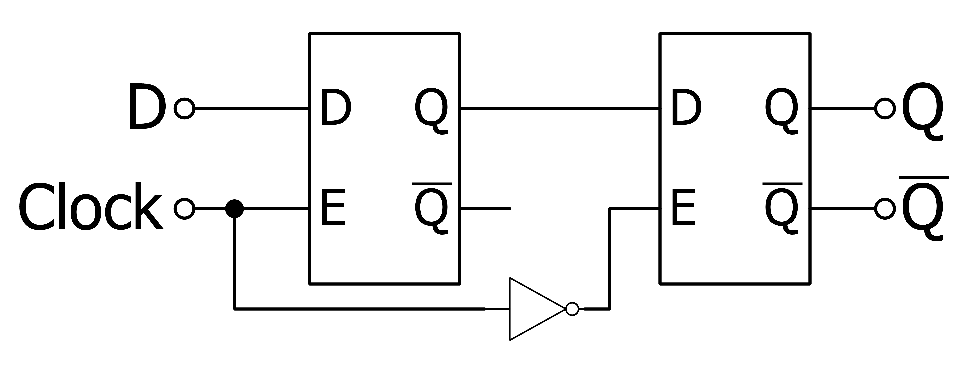
\includegraphics[scale=0.5]{D_FF.pdf}
        \end{center}
        \caption{Example of a Master-Slave D Flip Flop}
    \end{wrapfigure}
    \subparagraph{Master-slave flip flop} To make flip flops even more controllable we can put two in serial and make the second connected to $\overline{\texttt{clk}}$, in this way the flip flop will update on every falling edge of the clock (when the pulse goes from $\one\to\zero$).
    \section{Automata design} In combinatorial nets truth tables are what gives us the circuit's formalism, in the same fashion automatas are the equivalent for sequential nets. To describe the behaviour of FFs we indeed used \emph{extended} truth tables, but those can be made more intuitive through automata.
    \paragraph{Labelled Transition System} A labelled transition system (in layman's terms, an automata without outputs) is a quadruple $\langle Q, \Sigma, q_0, \delta\rangle$ where:
    \begin{itemize}
        \item $Q$ is a \emph{finite} set of states.
        \item $\Sigma$ is the input alphabet.
        \item $q_0$ is the starting state.
        \item $\delta= Q\times\Sigma\to Q$ is the transition function that defines all the relations \texttt{state/input} and to which next state they bring to. (It is a function, so for each $(q,i)\in Q\times\Sigma$ tuple there exists just one next state reachable!)
    \end{itemize}
    \paragraph{Mealy and Moore automata} Of course, since an LTS has no output it is indeed pretty useless in practical terms, to make it practical- to make it an automata, we define also a $\Delta$ output alphabet and a $\lambda$ function that we may add to the tuple (making it a sestuple) $\langle Q, \Sigma,\Delta q_0, \delta,\lambda\rangle$ such that:
    \begin{itemize}
        \item $\Delta$ is the output alphabet.
        \item $\lambda$ is the function defining the relations between output and states/transitions (we'll see it shortly).
    \end{itemize}
    The definition of the $\lambda$ function is somewhat problematic since it can be done in two ways giving two different types of automata:
    \begin{itemize}
        \item Moore automata: it relates states directly to outputs $\lambda:Q\to\Delta$
        \item Mealy automata: relating transitions to outputs $\lambda:Q\times\Sigma\to\Delta$
    \end{itemize}
    \paragraph{Equivalence between the two} Two automata of the same kind are said to be equivalent if, for the same sequence of inputs, they produce the same outputs. On the other hand, two different kind of automata are said to be equivalent if \emph{except for the first bit produced by the Moore automaton} they produce the same sequence of outputs (again, supposing the same sequence of inputs). How to prove this for \emph{any} automaton? The proof can be done either formally or empirically:
    \subparagraph{From Moore to Mealy} Their equivalence can be done formally by letting $M_1=\langle Q,\Sigma, \Delta, q_0, \delta, \lambda\rangle$ be the original Moore automaton and $M_2=\langle Q, \Sigma, \Delta, q_0, \delta, \lambda'\rangle$ be the equivalent Mealy automaton; as we can see their only difference is the function relating outputs- we can define $\lambda'$ such that:
    \begin{equation*}
        \lambda'(q,i)=\lambda(\delta(q,i))
    \end{equation*}
    In this way we are stating each output related to a transition in $M_2$ is equal to the output related to arrival states in $M_1$.
    In a more empirical way we can prove their equivalence by induction (even though it won't be practical), let $\sigma$ be any sequence of $n$ length of characters, if we can prove the equivalence between two different automaton on this sequence (in reality we should check any possible permutation of $\sigma$ through $\Sigma$) then we should also prove $n+1$ and then $n+2$ and so on (keep in mind that the sequence of the Moore automaton will have a first character that should not be considered for equivalence).
    \subparagraph{From Mealy to Moore} Their equivalence can also be done formally by letting $M_1=\langle Q,\Sigma, \Delta, q_0, \delta, \lambda\rangle$ be the original Mealy automaton and $M_2=\langle Q, \Sigma, \Delta, (q_0,b), \delta', \lambda'\rangle$ be the equivalent Moore automaton; in this case their difference is both the initial state (that is \emph{trivial} since the output character can be anything from the output alphabet, the important thing is that the equivalence works from the second output character in the sequence on) and the functions, that can be defined such that:
    \begin{equation*}
        \delta'((q, o),i), = (\delta(q, i), \lambda(q, i))
    \end{equation*}
    \begin{equation*}
        \lambda'((q, o)) = o
    \end{equation*}

    \paragraph{Automata minimization} The minimal automata equivalent of another one is said to be so if:
    \begin{enumerate}
        \item It is equivalent (\emph{sorry for the duh moment}).
        \item It is made up with the minimum amount of states possible.
    \end{enumerate}
    Why minimizing an automata you may ask? Because, since it has to be translated into a circuit, making the smallest possible automata is a fantastic way to reduce costs, physical space and complexity of the circuit.
    \subparagraph{Unreachable states} are those \emph{source} (see graph theory in programming) states that, if are not starting states, are unreachable since no composition of $(q, i)$ fed into $\lambda$ returns them. 
    \subparagraph{Indistinguishable states} two or more states are said to be indistinguishable if are reached by the same inputs and lead to the same states on the same inputs (this is not always true, they could be leading to different states that are themselves indistinguishable, another process to think about is a possible stalemate between 4 states where in pairs are indistinguishable apart from the fact that each of the pair leads to one of the other pair, thus creating an "endless" loop of dependencies).
    In a more general sense:
    \begin{itemize}
        \item In a Moore automaton two states are distinguishable if: the associated outputs are different or the outgoing transitions lead to distinguishable states.
        \item In a Mealy automaton two states are distinguishable if: their transitions return different outputs or they lead to distinguishable states.
    \end{itemize}
    \subparagraph{Algorithm for minimal automaton}
    \begin{enumerate}
        \item Delete unreachable states.
        \item Consider every possible pair of states and make a lower triangular table out of it.
        \item Check if each pair is trivially (have different outputs on the same inputs) distinguishable, note each non-trivially distinguishable pair with the pair that creates a stalemate (or already note them as indistinguishable if each pair leads to themselves).
        \item For each stalemate check that pair and look if that is already marked as distinguishable or indistinguishable, for the latter then the pair in stalemate is indistinguishable, for the other it is not and if nothing is reached put it aside and evaluate other pairs, go on until all stalemates are solved.
    \end{enumerate}
    From this triangular table we can derive the indistinguishability classes: two states are in the same class if and only if the pair associated to them is marked as indistinguishable in the table.
    A minimal automaton thus has:
    \begin{itemize}
        \item States formed by the indistinguishability classes.
        \item The initial state (derived from the original automaton)
        \item A transition function derived again from the original automaton that has to be reobtained by letting: $(class(q),i)\to class(q')$ whenever $(q,i)\to q'\in\delta$
        \item The output function on the other hand: for Moore the output of $q$ to the class of $q$, for Mealy the output of $(q,i)\to q'$ to the transition $(class(q),i)\to class(q')$
    \end{itemize}
    \section{Analysis of sequential nets} Analyzing a sequential circuit means to describe it using an automata:
    \begin{itemize}
        \item Identify the memory elements of the circuit (the Flip Flops).
        \item Identify (again) all the memory of the system given the status of the circuit.
        \item Compute the outputs produced by the system and the next memory state of the circuit for every possible state and input combination.
    \end{itemize}
    \subparagraph{Analysis procedure} We first need to analyze the combinatorial parts of the circuit such that to get all the boolean expressions for each variable (every input of each flip flop is a variable) and to get a truth table of them all, done that establish the future states of the circuit considering the the current states (all of them given by the truth table). Finally give symbolic names to every possible combination of bits stored in the flip flops, to every possible input sequence and to every possible output sequence. In the end infer the transitions and the output functions into an automaton. Lastly minimize the automaton, draw it and possibly give a verbal description of it.
    \subparagraph{Synthesis procedure} Like in a combinatorial net, the synthesis procedure is done such that to create a real digital circuit out of an "abstract" mathematical/graphical design. If not already done, from the verbal description we should get the automaton, from that (supposing it is already minimized) give binary encodings such that to cover all the possible states, the input and the output alphabets. From this derive a truth table containing the future states (thus an \emph{extended} truth table) and create entries for the input lines of all the needed flip flops (as many as there are bits needed to encode the states), decide which flip flop kind is the best by looking at its excitation table (if not specifically given). Finally derive from this table all of the needed boolean functions, possibly minimal. (Remember that how you decide to encode the states, the inputs and the outputs can matter on the efficiency of the design).
    \section{Registers}
    A register is an IC composed as a sequence of n flip flops, with them there are various technical issues that can be solved in multiple ways:
    \begin{itemize}
        \item Loading and unloading data.
        \item Implementing functionalities.
        \item Interconnecting them to each other (register's interconnections).
    \end{itemize}
    We first need to check the first issue:
    \subparagraph{PIPO, parallel input/parallel output} It is the simples kind of register, made out of flip flops of kind D, we just have to place them in line and, instead of feeding the clock directly to each of them, we first \texttt{AND} it to a \emph{load} signal, making it possible to decide when to store new data on the register.
    \subparagraph{SISO, serial input/serial output} These are made such that each flip flop gets its input from the previous one making it so the input line is just one and gets fed to the first flip flop and the output line is also one and is the ooutput of the last flip flop. Thus values are stored and unloaded each one at a time (each time the \emph{shift} signal is on and a descending wave front happens).
    \subparagraph{SIPO, serial input/serial output} Practically the same as a \texttt{SISO} register, but the outputs of each flip flop is sent as an output of the register.
    \subparagraph{PISO, parallel input/serial output} This is wildly different, it has both \emph{shift} and \emph{load} inputs (which we suppose can't be High at the same time) and, for the rest, does exactly what it says, it load parallely and outputs serially. There are multiple ways of making a PISO, but maybe the best one is where the clock is in \texttt{AND} with the \texttt{XOR} made from \emph{load} and \emph{shift} signals and the input of each FF is the result of a \texttt{MUX 2-to-1} controlled by the \emph{shift} signal where to value Low the line is equal to the parallel input of that flip flop and to value High the line is fed from the output of the previous flip flop (in case of the first flip flop we can choose to either connect it to $\texttt{V}_{\texttt{cc}}$, \texttt{GND} or another input, depends from the design).\\

    \noindent There exist multiple functions that can turn very useful to manipulate data and thus are neat to have in our registers.
    \paragraph{Shifter} It is a type of register able to shift values from right to left or from left to right, a right register is indeed the same as a SISO register, while a left register is a little bit more convoluted since values have to be sent backwards from the \texttt{MSB} to the \texttt{LSB}. We can even define a bidirectional shifter such that, adding a new input line \emph{right} it will work as a right shifter when that is High or as a left shifter when it is Low (again, we can use a \texttt{MUX 2-to-1} to do this very cleanely).
    \subparagraph{With holding} In some cases (like a 2-compl manipulation) we may want to keep the first or the last bits in their place when shifting in their other direction (by not doing that we would lose them because they would be pushed away to the following bit and not replaced by anything), thus we can define right, left and bidirectional shifters with holding (that we can also define as another input line, say \emph{hold}).
    \subparagraph{Circular registers} Finally we can also define circular shift registers such that the last and the first bit are reinserted from the other side of the register, we can thus define clockwise ($F_i\to F_{i-1}$) and counterclockwise ($F_i\to F_{i+1}$)registers (and likely bidirectional circular registers that can do both).
    \paragraph{Counter} A counter is a register used to count the number of occurrences of a certain event, always modulo something. Usually the modulo of a counter is based on it's number $n$ of flip flops, it is indeed equal to $2^n$. Tipically the countable events are clock's impulses or the occurrences of some input values or sequences. There exist two kind of counters, synchronous and asynchronous, in the first type all flip flops have the same clock while in the second one they have different ones. Both of the types can count upwise or downwise and some of them can be set to \emph{jump} to new values that does not attend the counting sequence, this property enables programmers to create loops and conditions.
    \subparagraph{Synchronous counter} We can synthetize a counter \texttt{mod $2^n$} pretty easily, it is done by letting each flip flop (we use \texttt{JK} ones) be $\texttt{J}_i=\texttt{K}_i=y_0\dots y_{i-1}$, on the other hand, if we are doing a downwise counter we have to use the complements of the outputs $\overline{y}$, from this we can even design a bidirectional counter, we just have to implement an \texttt{UP/DOWN} signal and feed it normally (as in the previous designs) to the upwise part of the circuit, while giving it complemented to the downwise part of the circuit, the two parts are just put in $OR$ to eachother everytime they have to be fed to the \texttt{JK} inputs.
    \subparagraph{Counter modulo k} These can be done solely (* we'll see in a moment)  by following a synthesis procedure, thus can be quite time intensive to make.
    \subparagraph{Counters of other things} These are very easy to make, just put the occurrence's High signal in \texttt{AND} with the clock and boom, you are done.
    \subparagraph{Asynchronous counter} Looking at the temporal diagram of a synchronous counter we can notice something: each flip flop $i$ toggles at every descending wave front of the previous one, this is huge because from this knowledge we can feed the output of each flip flop to the output of it's previous one- there is just one problem though, the values will take time to update, because the tau of each flip flop will sum to the other one. (of course downwise and bidirectional async counters are possible too, just feed the complemented previous flip flop's value into the clock of the next flip flop and you can go down!)
    \subparagraph{Delay propagation} During the increase phase in asynchronous counters we'll see a ripple effect where, during very small amounts of time, the values of the counter will not be right because they are still updating, in almost all applications this phenomenon can be ignored, but when doing really sensible circuits we should keep in mind this possible problem.
    \begin{wrapfigure}[9]{r}{0.3\textwidth}
        \centering
        \begin{tabular}{| l | c | c |}
            \hline
            & \texttt{P} & \texttt{C} \\\hline
            Normal FF & \zero & \zero\\
            immediate \texttt{RESET} & \zero & \one\\
            immediate \texttt{SET} & \one & \zero\\
            \texttt{-----} & \one & \one\\\hline
        \end{tabular}
    \end{wrapfigure}
    \vspace{-1cm}
    \subparagraph{Asynchronous inputs} Some flip flops are equipped with 2 more input lines called \texttt{PRESET} and \texttt{CLEAR}, these two special lines enable us to set or reset the flip flop instantaneously regardless of the clock status.
    \subparagraph{Modulo k counter} From this notion we can see how making a \texttt{mod} $k$ counter becomes very easy, just create a circuit returning 1 on the occurrence of the bits encoding $k$ and when it goes High reset the counter through an \texttt{all-CLEAR} signal going through all the flip flops.
    \subparagraph{Jumps in presettable counters} These kinds of counters are mostly used in program counters and, as previously said, enable us to keep track of the current evaluated line of code and work like this:
    \begin{itemize}
        \item If PL (a new signal line) holds \zero then they work as a normal upwise counter.
        \item If PL holds \one the register immediately stores values fed throgh pins $\texttt{P}_{n-1}\dots\texttt{P}_0$ in their respective flip flops, after PL goes \zero the counter returns to counting from the stored value.
        \item If we want to keep storing new values we just keep PL to \one.
    \end{itemize}
    \paragraph{Interconnections between registers} To be stored and handled throgh a circuit, information has to be moved from one register to another within the system: this is done through interconnection nets. (When using parallel output registers data is \emph{not moved}, because it remains in the source register, it is \emph{copied})
    We can define four different kinds of interconnections:
    \begin{center}
        \begin{tabular}{| l | c | c |}
            \hline
            & Fixed destination & Variable destination \\\hline
            Fixed source & \texttt{point-2-point} through logic gates & With decoders\\
            Variable source & With multiplexers & With meshes/buses\\
            \hline
        \end{tabular}
    \end{center}
    \subparagraph{Point to point interconnection, 1:1} This is really straightforward, it depends on what we want to do, but we can generalize everything by just saying to let the signal of the line \texttt{in\_R'} be High when we want to transfer data from register \texttt{R} to \texttt{R'}.
    \subparagraph{The buffer tri-state} Instead of using \texttt{AND} gates during the transfers of bits from \texttt{R} to \texttt{R'} (we should put the output bits of \texttt{R} in \texttt{AND} with \texttt{in\_R'} to store only when we intend to) it is usual to implement buffer tri-states, they have practically the same truth tables, but are inherently different on the technical level.
    \begin{center}
        \includegraphics{tristate.pdf}
    \end{center}
    \begin{itemize}
        \item Open circuit with $\texttt{B}=\zero\to\texttt{C}=\zero$
        \item Closed circuit with $\texttt{B}=\one, \texttt{A}=\zero\to\texttt{C}=\zero$
        \item Closed circuit with $\texttt{B}=\one, \texttt{A}=\one\to\texttt{C}=\one$
    \end{itemize}
    \subparagraph{Many sources to fixed destination with multiplexers, N:1} This interconnection too is fairly easy, we just need to select the register we want to take the data from and feed its code into the multiple multiplexers taking each bit of each register as input and outputting the right one, in the end we just also have to let \texttt{in\_R'} be High.
    \subparagraph{Fixed source to many destinations with decoders, 1:N} This can be quite tricky to think about because we could wrongly assume to use a demultiplexer to do this, but it is wrong because we would yes write into the right register, but would also clear all other registers in the process. To do this the right way just feed the outputs of the source register in all destination registers and choose where to write by making the \texttt{in\_R'} of each register a line coming from a decoder selecting on the basis of the code we give it.
    \paragraph{Galore of many sources to many destinations, N:N} To make many sources to many destinations interconnections is fairly easy (\emph{but oh my, complex/laborious to draw}), we just have to draw multiple many sources to fixed destination circuits\dots But we get into a problem with this: cost. You see, what I've now described is what we call a \emph{mesh}, it is \emph{very} fast, and is usually done such that every register is both a source and a possible destination, but it is also very costly since it uses a lot of multiplexers, because of this we may want to design other kinds of many to many interconnections that aren't as fast (namely they can't support parallel transfers from multiple sources) but are for sure smaller and many times cheaper.
    \subparagraph{A cheaper mesh} Through this design we can still use multiplexers but can't handle parallel transfers from multiple sources, we are going to use just \emph{one (fat)} multiplexer that has its output fed into every register input, in this way we can transfer the contents of one register into other multiple ones, but can do just one transfer at a time, we just have to handle the \texttt{in\_R}s of every register such that only the registers we want are written onto.
    \subparagraph{Using a bus} A bus is probably the cheapest choice, it is a \emph{single} (as always, since the bits in a register are many the real connections are multiple) that connect each register to every other one, it is made such that the outputs of the registers are fed into tri-state buffers that are controlled by dedicated $\texttt{from\_R}_{i}$ signal lines (that, watch out, can be High just one at a time- could be handled nicely through a decoder).
    \subparagraph{Wrap up memory} Meshes and buses are both used in computers, but each for different kinds of memory.
    \begin{itemize}
        \item In the central memory, the one of the microprocessor, there are very few registers and speed is preferable, because of this meshes are used.
        \item In mass storage there needs to be a big amount of space, thus buses are preferred.
    \end{itemize}
\end{document}